\documentclass{article}
\usepackage{graphicx} % Required for inserting images
\usepackage{enumitem}
\usepackage{xcolor}

\setlength{\oddsidemargin}{-0.25in}
\setlength{\topmargin}{-0.5in}
\setlength{\headheight}{0cm}
\setlength{\headsep}{0cm}
\setlength{\textheight}{10in}
\setlength{\textwidth}{7in}
\setlength{\topskip}{0cm}

\begin{document}

\noindent\textbf{ComS 472 - PS1 \quad Due: Sept 15, 2024 \quad Name: Aren Ashlock}

\begin{enumerate}

% ----------------------------------- 1 NOT DONE -----------------------------------

\item \textbf{(20 pts)} (Exercise 3.8) Give a complete problem formulation for each of the following. Choose a formulation that is precise enough to be implemented.

    \begin{enumerate}[label=($\alph*$)]
    
    % ----------------------------------- 1a DONE -----------------------------------
    
    \item \textbf{(5 pts)} Using only four colors, you have to color a planar map in such a way that no two adjacent regions have the same color.

    \color{blue}
        \textbf{States:} The states would show all the tiles, which color they are painted (if they are painted), and what tile you are on. \\
        \textbf{Initial State:} Any state can be the initial state, but I'll say that you are on the furthest left and top tile and all the tiles are unpainted. \\
        \textbf{Actions:} There are 8 actions that can be taken such as move left, right, up, or down, or you can paint the current tile 1 of the 4 colors. \\
        \textbf{Transition Model:} Choosing to paint the current tile changes the color of the state to a different state with the corresponding tile color (unless the tile is painted the same color it already was, which it would then transition to the same state it was already in). If you attempt to move in any of the directions and there is a tile in that spot, there will be a transition to a state that shows you on the new tile. If you attempt to move to a spot where there is no tile, the transition maps back to the current state. \\
        \textbf{Goal State(s):} All states in which no two adjacent regions are painted the same color. \\
        \textbf{Action Cost:} Each action costs 1.
    \color{black}

    % -------------------------------------------------------------------------------

    % ----------------------------------- 1b DONE -----------------------------------

    \item \textbf{(5 pts)} A 3-foot-tall monkey is in a room where some bananas are suspended from the 8-foot ceiling. He would like to get the bananas. The room contains two stackable, movable, climbable 3-foot-high crates.

    \color{blue}
        \textbf{States:} Each state shows the room including how many bananas are on the ceiling, the number of bananas the monkey has, where the two crates are, and the location of the monkey. \\
        \textbf{Initial State:} Once again, any state can be the initial state. However, I would imagine the monkey is somewhere on the ground, the crates are in an arbitrary location, and there is some amount of bananas suspended from the ceiling. \\
        \textbf{Actions:} First off, the monkey can move forwards, backwards, left, right, or climb a crate. Also, the monkey can turn right or left. In addition to movement, the monkey can grab or place a crate. Finally, the monkey can grab a banana from the ceiling. \\
        \textbf{Transition Model:} Almost every action transitions to a new/different state (the monkey is in a different spot vertically or horizontally, the crates are picked up/moved/put down, or there are less bananas on the ceiling and more in the monkey's possession). The only exception is if the monkey attempts to move forward or backward into a wall, which would result in the state staying the same. \\
        \textbf{Goal State(s):} All states where the monkey has all the bananas. \\
        \textbf{Action Cost:} Each action costs 1.
    \color{black}

    % -------------------------------------------------------------------------------

    % ----------------------------------- 1c DONE -----------------------------------

    \item \textbf{(5 pts)} You have a program that outputs the message “illegal input record” when fed a certain file of input records. You know that processing of each record is independent of the other records. You want to discover what record is illegal.

    \color{blue}
        \textbf{States:} All the possible states are each file as either illegal, legal, or unknown (yet to be scanned). \\
        \textbf{Initial State:} It could be any state as an initial state, but a good one is all files are unknown. \\
        \textbf{Actions:} Each action is scanning which file. \\
        \textbf{Transition Model:} After scanning a file, the state always transitions to either a state which the file is legal or illegal. \\
        \textbf{Goal State(s):} The goal state is the one where you feed a certain file of input records and the output is "illegal input record" (which there should only be 1 goal state then) \\
        \textbf{Action Cost:} Each action costs 1.
    \color{black}

    % -------------------------------------------------------------------------------

    % ----------------------------------- 1d DONE -----------------------------------
    \item \textbf{(5 pts)} You have three jugs, measuring 12 gallons, 8 gallons, and 3 gallons, and a water faucet. You can fill the jugs up or empty them out from one to another or onto the ground. You need to measure out exactly one gallon.

    \color{blue}
        \textbf{States:} The possible states are all the different levels of fullness the jugs are. The fullness of all 3 jugs combine to a singular state. \\
        \textbf{Initial State:} As mentioned in the other 3 problems, there could be any initial state. I'd say a good initial state is all 3 jugs are completely empty. \\
        \textbf{Actions:} The agent can either choose to fill up a jug, empty 1 jug into another, or empty a jug onto the ground. \\
        \textbf{Transition Model:} Most every action will transition to another state which has a different combination of water levels in all 3 jugs. However, if the agent chooses to fill a jug that is already full or empty out a jug that's already empty, it stays in the same state. \\
        \textbf{Goal State(s):} The goal states are any in which any of the 3 jugs contains exactly 1 gallon. \\
        \textbf{Action Cost:} Each action costs 1.
    \color{black}

    % -------------------------------------------------------------------------------
    
    \end{enumerate}

% ----------------------------------------------------------------------------------

% ------------------------------------- 2 DONE -------------------------------------

\item \textbf{(10 pts)} (Exercise 3.7) The n-queens problem, informally introduced in the textbook, is defined on page 12 of the PPT lecture notes titled ”4b. problem solving.pptx”, which was posted on September 4. Consider the $n$-queens problem using an “efficient” incremental formulation given below.

\begin{itemize}
    \item \textit{States:} All possible arrangements of $k$ queens (0 $\leq k \leq$ n), one per column in the leftmost $k$ columns, with no queen attacking another.
    \item \textit{Initial state:} No queen on the board.
    \item \textit{Actions:} Add a queen to any square in the leftmost empty column such that it is not attacked by any other queen.
\end{itemize}

Explain why the state space has at least $\sqrt[3]{n!}$ states. Also, estimate the largest $n$ for which exhaustive exploration is feasible, assuming that the most powerful supercomputer can process 200,000 trillion calculations per second. (\textit{Hint:} Derive a lower bound on the branching factor by considering the maximum number of squares that a queen can attack in any column.)

\color{blue}\textbf{Answer:} The state spaces is at least $\sqrt[3]{n!}$ states because when we place a queen, it can attack up to 3 squares in any column. Because of that, the permutation would go $n \times (n-3) \times (n-6) \times ...$, which results in $\sqrt[3]{n!}$ as a lower bound for the number of states. As for the largest $n$, 200,000 trillion becomes $2 \times 10^{17}$, which cubing results in $8 \times 10^{51}$ and the closest factorial is $42!$. Therefore, $n = 42$ is the largest $n$. \color{black}

% ----------------------------------------------------------------------------------

% ------------------------------------- 3 DONE -------------------------------------

\item \textbf{(10 pts)} Suppose 8-puzzles have the same goal state $S_g$ shown below.

\begin{center}
    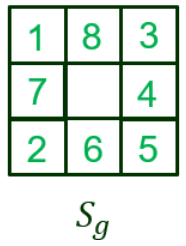
\includegraphics[scale=0.75]{472-PS1-Q3-Sg.png}
\end{center}

\begin{enumerate}[label=($\alph*$)]
    
    % ----------------------------------- 3a DONE -----------------------------------
    
    \item \textbf{(4 pts)} How many inversions are in $S_g$?

    \color{blue}\textbf{Answer:} $0+6+1+4+1+0+1+0 =$ \textbf{13 inversions} \color{black}

    % -------------------------------------------------------------------------------

    % ----------------------------------- 3b DONE -----------------------------------

    \item \textbf{(6 pts)} Consider two 8-puzzles respectively with the initial states $S_1$ and $S_2$ below. Are these puzzles solvable? Please explain.

    \begin{center}
        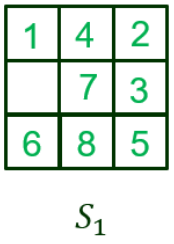
\includegraphics[scale=0.75]{472-PS1-Q3-S1.png} \hspace{5 cm} 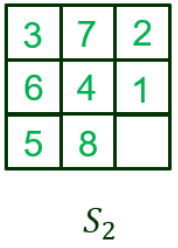
\includegraphics[scale=0.75]{472-PS1-Q3-S2.png}
    \end{center}

    \color{blue}\textbf{Answer:} In both instances, the number of inversions in the goal state is 7. For $S_1$, there are 7 inversions. That results in a difference of 0, which is even. Since the difference is an even number, it ($S_1$) \textbf{is solvable}. As for $S_2$, there are 12 inversions. For this grid, we get a difference of 5, which is odd. When the difference is an odd number, it ($S_2$) is \textbf{not solvable}. \color{black}

    % -------------------------------------------------------------------------------
    
    \end{enumerate}

% ----------------------------------------------------------------------------------

\end{enumerate}
\end{document}